\documentclass{article}

% Language setting
% Replace `english' with e.g. `spanish' to change the document language
\usepackage[english]{babel}
\usepackage{cite}
% Set page size and margins
% Replace `letterpaper' with `a4paper' for UK/EU standard size
\usepackage[letterpaper,top=2cm,bottom=2cm,left=3cm,right=3cm,marginparwidth=1.75cm]{geometry}

% Useful packages
\usepackage{amsmath}
\usepackage{graphicx}
\usepackage[colorlinks=true, allcolors=blue]{hyperref}

\title{MapReduce Introduction and Implementation}
\author{Zifan WANG, Yazhou SHEN}

\begin{document}
\maketitle

\begin{abstract}

MapReduce \cite{dean2008mapreduce} is one of the most popular programming models that was developed by Google ten years ago. This model employs map and reduce functions, operating on $<key, value>$ pairs as input and output to get closer to the final result step by step. All programs written in that specific style can run distributed and parallel through the MapReduce framework. Parallellization of the framework accelerate the 
execution while distribution make the framework scalable and can handle infinite number of data as long as we have enough machines.

We go through paper that introduce MapReduce as well as papers that gives a clear definition of MapReduce class and proves the correctness of the MapReduce in order to gain a deep understanding of this framework.
We also utilize socket programming to build our own MapReduce framework in python and evaluate its complexity.


\end{abstract}

\section{Introduction}
We amidst an era characterized by an explosion of information, where the daily processing of vast datasets has become a necessity. 
Computation power is much more valuable than ever. And due to physics limit, people cannot keep reducing the size of semi-conductors' size and challenging the perpetuity of Moore's Law.  Consequently, the relentless enhancement of computational power in a single machine becomes unattainable. This has prompted a shift in focus towards multiple-machine computation systems, where numerous nodes collaborate to accomplish common tasks.
MapReduce, developed by Google, is designed to process large volumn of data. There are mainly three steps in MapReduce framework including: Map, Reduce, Shuffle. Basically each round of Map to Shuffle to Reduce will be 
a straightforward computation and users can get final result from original input after multiple rounds of simple execution. With MapReduce framework,
program written in specific paradigm can be automatically parallelized and distributed. MapReduce achieves remarkable performance with a relative simple structure.

In this report, we present basic introduction of MapReduce including its structure, execution overview, framework correctness and algorithm design principle. Besides, we 
will also present our own implementation of MayReduce. We utilize python and socket programming as the main tool and how we try to realize the basic function of MapReduce including: Map, distributed shuffle, reduce as well as basic fault tolerance.
We also analyze the time complexity of our implementation.


\section{Programming Model \cite{dean2008mapreduce}}
There are two main functions in MapReduce framework: Map
and Reduce. Another function called Shuffle is between Map and Reduce phase that do some intermediate data process.
Map function  process input $<key, value>$ pairs and generate a set
of intermediate $<key, value>$ pairs. The Shuffle function groups the generated
$<key, value>$ pairs altogether by the same key, and passes them to the Reduce
function. Then for the Reduce function, it receives an intermediate key and a
set of values for that key. Then it merges these values to form smaller set of
values. The Map and Reduce functions are defined
by users, so it is actually highly customizable, as long as it follows the basic
paradigm.
\section{Structure}
\begin{figure}
      \centering
      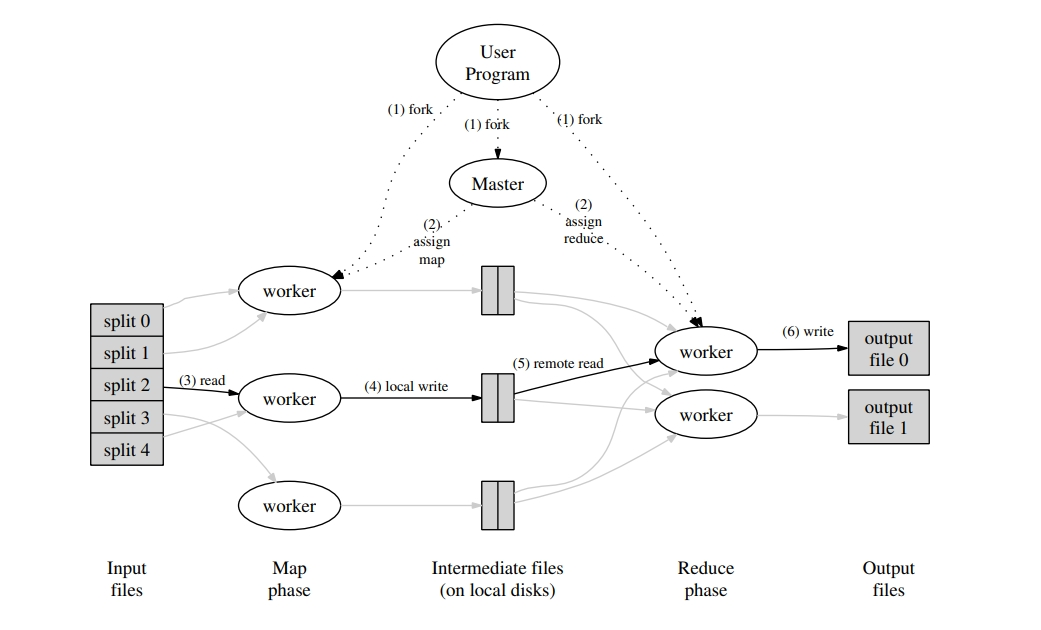
\includegraphics[scale = 0.4]{structure.png}
      \caption{MapReduce Structure \cite{dean2008mapreduce}}
\end{figure}
\subsection{Execution Overview \cite{dean2008mapreduce}}
The Map invocations are distributed across multiple
machines by automatically partitioning the input data
into a set of M(number of mapper) splits. The input splits can be processed in parallel by different machines. Reduce invocations are distributed by partitioning the intermediate key
space into R(number of reducer) pieces using a partitioning function (e.g.,
hash(key) mod R). The number of partitions (R) and
the partitioning function are specified by the user.
Figure 1 shows the structure and execution overview of a MapReduce operation. The detailed steps are as follows:

\begin{enumerate}
      \item MapReduce will first split the original input data to M pieces and transfer 
      the mapper.py and reducer.py to all the workers.
      \item There is a special machine among all the nodes called master that will coordinate the whole cluster.
       Master will assign work to rest of the workers. There will be M map tasks and R reduce
      tasks to assign. The master picks idle workers and
      assigns each one a map task or a reduce task.
      \item The mapper(worker with map task) read one split of the input data 
      that distributed to itself by master. The mapper will execute the mapper.py provided by 
      user and generate a list of $<key, value>$ pairs. Those pairs normally stored in memory if the memory is enough.
      \item The key value pair generated by mapper will hash to R regions that pairs in each region prepared for one reduce jobs.
      Workers will transfer the location of those R region to the master and wait for reducers to get those data. 
      \item After all the mapper finish execution and send the data location to master,
      reducer will be notified by the master about locations of data reducer need. In this step the MapReduce framework
      can guarantee that all  $<key, value>$ pairs with same key can go to the same reducer to guarantee the correctness.After reducer
      fetch those data, it sorts those pairs by the keys and make sure the pairs with same key are next to each other. If the intermediate data is too large,
      the framework can divided it into sub-reduce tasks and merge them together later.
      \item The reducer will run the reduce.py defined by user and merge the pairs with the same key together.
      The output of the Reduce function will be part of the final result that sent to user.
      \item When all map tasks and reduce tasks have been
      completed, the master wakes up the user program and return the result.
\end{enumerate}

\subsection{Fault Tolerance}

Fault tolerance is an important part in MapReduce framework since we need to deal with a large number of cluster. 
Even the probability of hardware failure 
of single machine is very low, we need to multiply it with number of machines in the cluster and failure is inevitable.

There are basically two kinds of failure in MapReduce framework.
\begin{itemize}
      \item Worker failure
      In order to check worker status, MapReduce framework use heartbeats algorithm that pings every worker periodically. No response from worker means the 
      worker met some issue. The map tasks running on that machine will be re-assigned to other idle workers. Similar for reduce jobs. 
      \item Master failure
      For simplicity, MapReduce framework will re-execute the entire job if it meet master failure. Since there will be only one single master,
      the probability to meet this failure is very low.
\end{itemize}

\section{System Evaluation}
MapReduce almost finish all the computation task for 
Google ten years ago but recently no one in Google write MapReduce program anymore.
 It is replaced by Flume and MillWhell$($Cloud Dataflow/Apache Beam$)$. We want to analyze MapReduce's advantage and disadvantage in this section.

\subsection{Advantage}
\begin{itemize}
      \item Scalability:
      MapReduce is highly scalable. Theoritically, we can keep increasing the number of machines in the cluster to store massive amount of data and process those
      data.
      \item Fault Tolerance:
      By utlizing the fault tolerance algorithm we discussed above, MapReduce is resilient for even large number node failure by redistributed and re-executing tasks, which is 
      also an important characteristic for large scale data processing.
      \item Parallel Processing:
      MapReduce enables parallel processing of data. The "map" phase processes data independently across multiple nodes,
       and the "reduce" phase consolidates the results in parallel, leading to efficient utilization of resources.
      \item Simplicity:
      MapReduce abstracts the complexity of distributed computing, making it easier for 
      developers to focus on the logic of their computations. The programming model simplifies the development of distributed applications.
      \item Flexibility:
      MapReduce is flexible and can handle various types of data processing tasks, 
      including batch processing, log analysis, and data transformation. It is not limited to a specific type of application.
\end{itemize}


\subsection{Disadvantage}
\begin{itemize}
      \item Programming Complexity:
      Despite its simplicity compared to traditional distributed computing models, MapReduce programming can still be complex for certain tasks. Developers need to design their algorithms in a way that fits the map and reduce paradigm.
      \item Latency:
      MapReduce is designed for batch processing and may not be suitable for low-latency applications. The framework introduces overhead due to the two-phase structure (map and reduce), making it less suitable for real-time processing.
      \item Data Movement Overhead:
      Moving large amounts of data between nodes during the map and reduce phases can result in significant data movement overhead. This can affect performance, especially when dealing with large datasets.
      \item Limited Support for Iterative Algorithms:
      MapReduce is less efficient for iterative algorithms (e.g., machine learning algorithms with multiple iterations) as it involves reading and writing to distributed file systems after each iteration.
      \item Not Suitable for All Types of Problems:
      While MapReduce is versatile, it may not be the best solution for all types of problems. Some algorithms and computations may not fit well into the map and reduce paradigm, leading to inefficiencies.
\end{itemize}

\section{Correctness Analysis}
\subsection{Definition of the MapReduce Class}
      \cite{model} introduces a formal definition of the MapReduce class follow three guiding principles:
      \begin{enumerate}
            \item Memory: "The input to any mapper or reducer be substantially sublinear in the size of the data" \cite{model} and it is $O(n^{1-\epsilon})$ .
            \item Machine number: The machine number be substantially sublinear in the size of the data to make it practical and make it to be $\Theta(n^{1-\epsilon})$ .
            \item Time: We only consider the mapper and reducer function can be finished in polynomial time with the original input length.
      \end{enumerate}

      \subsubsection{Formal Definition \cite{model}}

      Let $\epsilon > 0$. An algorithm in $MRC^i$ consists of a sequence $<\mu_1,\rho_1,\mu_2,\rho_2,\cdots, \mu_R,\rho_R,>$
      \begin{itemize}
            \item Each $\mu_R$ is a randomized mapper implemented
            by a RAM with O(log n)-length words, that uses
            $O(n^{1-\epsilon})$ space and time polynomial in n.
            \item Each $\rho_R$ is a randomized reducer implemented
            by a RAM with O(log n)-length words, that uses
            $O(n^{1-\epsilon})$  space and time polynomial in n
            \item the total space used by all the $<key,value>$ pairs is $O(n^{2-2\epsilon})$.
            \item The number of rounds R = $O(log^in)$ 
      \end{itemize}
      \subsubsection{Discussion}
      Since both map and reduce function running on polynomial algorithm with input or output size limited in the definition. We only worry about whether we will
      exceed memory limit during shuffle phase.


      Now we prove this lemma:
      Consider round r of the execution of an
      algorithm in MRC. Let $K_r$ be the set of keys in $U'_r$ let $V_r$ be the multiset of values in $U'_r$
      , and let $V_{k,r}$ denote
      the multiset of values in $U'_r$
      that have key k.
      Then Kr and Vr can be be partitioned across $O(n^{1-\epsilon})$ machines such that all machines get  $O(n^{1-\epsilon})$ 
      bits, and the pair $<k, V_{k,r}>$  gets sent to the same machine.

Proof. let s(B) denote the total space used by strings in B. So, due to total space limitation in the definition
$$s(V_r)+s(K_r) \leq O(n^{2-2\epsilon})$$
Because for any single machine in the definition, the total space is limited to $O(n^{1-\epsilon})$, so for all keys,we have 
$$|k|+ s(V_{k,r}) = O(n^{1-\epsilon})$$.
By use a Greedy algorithm similar to the greedy scheduler we talk about in class, the total space we need to have for shuffle phase is 
at most the average number of total space in addition to the largest space of single key. Therefore,
$$\leq \frac{s(V_r)+s(K_r)}{\text{num of machines}} + max(|k| + s(V_{k,r}))$$
$$\leq \frac{O(n^{2-2\epsilon})}{\Theta(n^{1-\epsilon})}+O(n^{1-\epsilon})$$
$$\leq O(n^{1-\epsilon})$$
Hence it will not exceed the memory limitation.
Therefore we proved the correctness of MRC that the execution of algorithm in our definition will not exceed the memory limit.
\subsection{Algorithm Design Technique for MRC}
In this section, we will introduce a class of algorithm that can be run efficiently in MRC.
\subsubsection{Definition \cite{model}}
We call a function f MRC-parallizable if there are functions g and h such that:
\begin{enumerate}
      \item For a random partition${T_1,T_2,\cdots,T_k}$ of S such that$\cup_iT_i = S$ and $T_i \cap T_j = \emptyset $
      for $i \neq j$ $f(S) = h(g(T_1),g(T_2),\cdots,g((T_k)))$
      \item $g$ and $h$ can be expressed in $O(log(n))$ bits
      \item $g$ and $h$  can be computed in time polynomial in $|S|$
      and every output of $g$ can be expressed in $O(log n)$
      bits
\end{enumerate}
In \cite{model}, it proves three lemma to make sure the algorithm under previous definition can be efficiently parallizable under memory restriction we disscused earlier.


\section{Implementation }

\href{https://github.com/beiduqiu/549_MapReduce.git}{Github page}


In our project, we implemented a simple MapReduce framework, which can execute basic MapReduce tasks. It can execute the users' tasks in a parallel and distributed way, and optimize the parallelism of original users' task.

(After the previous presentation, we have been working on reconstructing the framework to add the mechanism of \textbf{\textit{continuous listening}}. This is for the purpose to add fault tolerence. But our approach of communicating with socket causes a serious blocking and concurrency to our final framework, which unfortunately leads to the failure of our latest approach. We have been working on this for too much time, and still cannot solve it. A distributed file system may solve this problem, But in our practice, it is too complicated and time consuming for us to build a DFS, when we have already built the MapReduce framework first. However, for our new framework we have done unit tests on different key components, such as \textbf{\textit{Map}}, \textbf{\textit{Shuffle}} and \textbf{\textit{Reduce}}. And they can work correctly.)

Our framework is highly customizable, which means it can be applied to all the problems that user defines. A user of this framework just needs to prepare the $mapper.py$, $reducer.py$ and $data.txt$ following a few rules (the format of input/output), and send them to the server for distribution. The server will send the files to the worker machines for processing, and the user does not need to care how the inside mechanism is implemented. This allows a user who has limited knowledge in parallel and distributed computing to have access to distributed computing resources. And this is actually following the merit of the original MapReduce library by Google, that this framework is easy to use and user-friendly.

The framework consists of a master server and several worker machines. The server is responsible for communication coordination, and will not execute any direct data process (except the data split). We defined two classes for the server and workers. Each machine in this cluster only needs to spawn an object of the corresponding class.



According to the different phases, we divide the introduction of our framework into the following parts:
	\subsection{Setup}
		First, a master server needs to know how many worker machines are there to be used. Then the server will use a for-loop to listen the connection requests from the worker machines. Meanwhile, the worker machines are activated and send connecting requests to the server through socket. Once a connection between server and worker is set up, the server will restore the socket into a data strucutre, and set the state of the worker to a default $idle$. When all the worker machines are ready, the server send the files as well as a list of the addresses of the workers to each worker machine, and set the states of the workers to $mapping$ in the data structure.
	
	\subsection{Map}
		When a worker receives all the files and information it needs, it becomes a \textit{Mapper}. (Its state is set to be $mapping$ on the server side). It will directly run the $mapper.py$ and save the output of <key, value> pairs to a $mapped.csv$ file.
	
	\subsection{Shuffle}
		After a worker finishes the \textit{\textbf{Map}} process, it will sort the <key, value> pairs on its local, and hash the keys into a bucket structure, according to the total number and worker ID of the machines. Then according to the bucket structure, the $mapped.csv$ will be split into several parts. After all of these are done, the worker machines will send a signal to the server, which is keeping listening ever since the \textit{\textbf{Setup}} phase is finished. The server will switch the state to $idle$ from $mapping$ of the worker machine, after its signal is received. Once all the workers are $idle$ again, the server will send a signal $reduce$ to all of the workers, and switch their states to $reducing$. Likewise, it will keep listening to their responses. The workers will then do the following at the same time: sending the split mapped files to other corresponding workers, and receive files from them. This is done by $threading.Thread()$ function in Python. Again, after all of these are done, the worker sends a signal to the server, which will set the states to $idle$. The result of this phase is that, now every worker has different files from other workers, in which there are the <key, value> pairs this worker needs to do.
		
		Beside of the implementation above, we also implemented a distribution sort version of the shuffling. When the workers stop the mapping phase, and send the signals to inform the server, the server will call a distribution sort by $dask$ libaray in Python to shuffle the <key, value> pairs. However, the results should be restored either on the server or a distributed file system, which is not compatible with our framework. In this case, we did not use this version of \textbf{\textbf{Shuffle}}.
		
	\subsection{Reduce}
		Once all of the workers are $idle$ in the data structure on the server side, the server will send the $reduce$ signal to the workers, and switch the states to $reducing$. When a worker receives the signal, it will first call a $combine()$ function to concatenate the mapped files into one. Then it will execute under the reducing logic to get the final result from this file, and restore the results into a $reduced.csv$.
	
	\subsection{Other Details}
		In our implementation, one rule that the users need to follow is that the <key, value> pairs are restored in the type of $<pandas.DataFrame>$, with two columns named $Key$ and $Value$. This is for the consideration of easier and efficient data processing with Python language. Another rule that user should follow is to print the outputs of the $mapper.py$ and $reducer.py$ directly into the console. The framework can save the prints in the consoles to logs. In general, a user does not need to know much pre-knowledge of the framework, and many format issues can be addressed by directly calling functions we provide in $utils.py$.
		
		In our implementation, we follow such an asumption that the worker machines are specificly used for the MapReduce cluster, under the same network. Every worker machine knows the address of the address.
		
(After the previous presentation, we have been working on reconstructing the framework to add the mechanism of \textbf{\textit{continuous listening}}. This is for the purpose to add fault tolerence. But our approach of communicating with socket causes a serious blocking and concurrency to our final framework, which unfortunately leads to the failure of our latest approach. We have been working on this for too much time, and still cannot solve it. A distributed file system may solve this problem, But in our practice, it is too complicated and time consuming for us to build a DFS, when we have already built the MapReduce framework first. However, for our new framework we have done unit tests on different key components, such as \textbf{\textit{Map}}, \textbf{\textit{Shuffle}} and \textbf{\textit{Reduce}}. And they can work correctly.)

\section{Analysis}
In this part, we are going to analyze the performance and problems of our MapReduce Framework.
	\subsection{Complexity}
		In our framework, the whole MapReduce tasks will be divided into the following stages (suppose there are N machines, the whole $data.txt$ has a length of M, and K different keys):
		\begin{itemize}
			\item \textbf{Setup: }This part includes connecting and task assigning. Suppose a connection takes an average of $T_{con}$ time, and an average of $T_{send}$ for sending user files, and the time cost of machine activation can be ignored. Since our server uses a sequential for-loop to do so, it takes $T_{Setup}=N\times (T_{con} + T_{send}).$
			\item \textbf{Map: }Suppose executing user's $mapper.py$ takes $T_{m}$. The time cost of logging from the console, and sending/receiving signals can be ignored. The sorting takes $O(\frac{M}{N}\lg \frac{M}{N})$. Thus $T_{Map}=T_{m}+O(\frac{M}{N}\lg \frac{M}{N})$.
			\item \textbf{Shuffle: } Suppose the time of sending/receiving signals can be ignored. The hashing takes $O(\frac{K}{N})$ in average (if balanced). and the sending/receiving takes $(N-1)\times max\{ T_{sned^{'}}, T_{receive^{'}}\}$. Thus $T_{Shuffle}=O(\frac{K}{N})+(N-1)\times max\{ T_{sned^{'}}, T_{receive^{'}}\}$ in a key-balanced case.
			\item \textbf{Reduce: } Suppose executing user's $reducer.py$ takes $T_{r}$. The time cost of combining the mapped files can be ignored. It is hard to analyze the time cost of reducing, but in an ideal work balanced case, it takes $O(\frac{M}{K})$. Thus $T_{Reduce} = T_{r} + O(\frac{M}{K})$.
			
		\end{itemize}

	\subsection{Problems}
		The framework is still far from an efficient framework, and there are still many issues we have not addressed yet. Here we list some of the problems we noticed during our implementation, but failed to fix for some reasons.
			\begin{itemize}
				\item \textbf{High Network Traffic: }In our implementation, we have not optimized the communication effectively yet. This causes an extremely high load to the network. For example, during a \textit{\textbf{Shuffle}} phase, the workers are connected to all of the other machines, which becomes a dense network. In this case, the framework could not be compatible once the number of machines are large. This can be alleviate with the help of a distributed file system, which is too complicated for our framework.
				\item \textbf{Fault Tolerence: } In our final version of the framework, we did not include the fault tolerence mechanism, because combined with our mechanism of \textit{continuous listening}, it will be too complicated to implement. (Although we have restored a data structure of tasks for this purpose.) However we are fully aware of the potential risk, when a machine dies, its works will fail, and extend the total time cost of the whole MapReduce task.
				\item \textbf{Unbalanced Workload: } In our implementation, during a \textit{\textbf{Shuffle}} stage, we simply divide the keys via a bucket structure with hash. However, we ignored the problem that different bucket may have different keys, which may potentially lead to a worker to deal too much <key, value> pairs, which another one may have nothing to do. Moreover, the number of pairs of different keys may also be unbalanced.
				\item \textbf{Lack of Parallelism: } Admittedly, in our implementation we still used too much sequential methods to process the tasks. For example, our server uses a sequential for-loop to connect with workers, which can actually be replaced by a parallel for-loop. If more parallel methods are added, the whole framework can be further optimized.
\end{itemize}

\bibliographystyle{IEEEtran}
\bibliography{IEEEexample}

\end{document}